\documentclass[a4paper,10pt]{article}
\usepackage[T1]{fontenc}
\usepackage[utf8]{inputenc}
\usepackage{lmodern,textcomp}
\usepackage[margin=2.2cm]{geometry}
\usepackage{amsmath,amssymb,siunitx,booktabs,graphicx,tabularx,array,enumitem,xcolor,fancyhdr,float}
\usepackage[colorlinks=true,linkcolor=blue!50!black,urlcolor=blue!50!black]{hyperref}
\setlength{\parindent}{0pt}
\setlength{\parskip}{4pt}
\setlength{\headheight}{14pt}
\renewcommand{\arraystretch}{1.2}
\renewcommand{\tabularxcolumn}[1]{>{\raggedright\arraybackslash}p{#1}}
\setlist{nosep,leftmargin=*}
\newcommand{\file}[1]{\nolinkurl{#1}}
\sisetup{per-mode=symbol}
\pagestyle{fancy}\fancyhf{}
\fancyhead[L]{34870 Electroacoustics}
\fancyhead[R]{Lab C --- Microphone calibration}
\fancyfoot[L]{Group 10 \quad / \quad measured 29 September 2026}
\fancyfoot[R]{\thepage}
\graphicspath{{../figures/}{Lab C/figures/}{../ltspice/}{Lab C/ltspice/}}
\begin{document}
\begin{center}
{\Large\bfseries Lab D --- Loudspeaker Impedance and Near Field}\\[5pt]
34870 Electroacoustics\\[4pt]
Group 10: Louis Andrianne, Sophie Kimura, Mads Rudolph\\[4pt]
Measured Tuesday 6 October 2026, building 354, room 026
\end{center}
\thispagestyle{fancy}

\section{Purpose and Setup}

The three main objectives of this lab are to measure the impedances of the driver units in the loudspeaker system for the project, derive the Thiele-Small parameters for the woofer unit, and illustrate the low frequency effects of the boxed loudspeaker. This will be done by first measuring the DC resistance of each driver. Next, the electrical input impedance is measured for the tweeter, midrange, and open-vent woofer. The Thiele-Small parameters of the woofer are then examined for setups with free air and with a closed box. The influence of the vent is specifically examined by carrying out measurements with varying vent lengths. Lastly, the near field responses of the woofer unit and vent are measured in order to assess low frequency responses.\\

\textit{Info on setup and equipment}


\section{Part 1: DC Resistance}
The DC resistance of each of the drivers is measured to investigate the electrical resistance of the voice coil wires. This is done by connecting a multimeter to the two terminals of the voice coil, which sends out a small voltage and measures the returning current to calculate resistance. These results can be seen in Table \ref{tab:DC}\\



\begin{table}[H]
    \centering
    \begin{tabular}{c|c|c}
        $R_E$ Tweeter [$\Omega$]& $R_E$ Midrange [$\Omega$]& $R_E$ Woofer [$\Omega$] \\
        \hline
        3.4  & 4.6 & 5.7\\
    \end{tabular}
    \caption{Measured DC resistance}
    \label{tab:DC}
\end{table}



\section{Part 2: Electrical Input Impedance}

The input electrical impedance is measured for each of the drivers. The loudspeaker is connected to the amplifier output through a circuit connection board which contains a resistor in series. Additionally, connectors for measuring voltages for the amplitude and loudspeaker, $V_{amp}$ and $V_{speaker}$, respectively, are attached to the board. This setup is shown in Figure \ref{fig:impedance_setup}.\\


\begin{figure}[H]
    \centering
    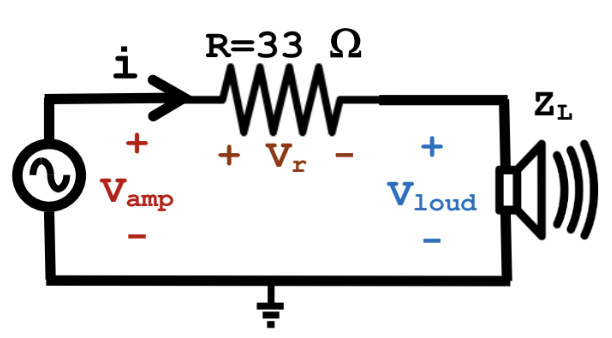
\includegraphics[width=0.5\linewidth]{Lab D/figures/impedance_setup.png}
    \caption{ Circuit connection board}
    \label{fig:impedance_setup}
\end{figure}

This setup allows us to measure the voltage difference across the loudspeaker and the voltage of the amplifier. We use this to calculate the resistor voltage $V_{R}$. Our circuit uses a resistor with a known resistance in order to calculate the current through the circuit $I$. With $I$ and $V_{speaker}$, we are then able to solve for the impedance of the loudspeaker, $Z_{loudspeaker}$.

\begin{align}
    V_R &= V_{amp} - V_{loudspeaker}\\
    I &= \frac{V_R}{R}\\
    Z_{loudspeaker} &= \frac{V_{loudspeaker}}{I}\\
    & = \frac{V_{loudspeaker}}{\frac{V_R}{R}}\\
    & = R (\frac{V_{loudspeaker}}{V_{amp} - V_{loudspeaker}})\\
    & = R(\frac{\frac{V_{loudspeaker}}{V_{amp}}}{1 - \frac{V_{loudspeaker}}{V_{amp}}})
    \label{eq:DC}
\end{align}

These measurements are recorded with the following methods. The targeted frequency range is covered with the multitoned signal generated by the NI 4431 and sent to the amplifier. The amplifier receives this input from the output channel AO0 of the NI 4431. The amplifier output $V_{amp}$ is then fed into channel AI0 of the NI 4431. The loudspeaker excitation signal $V_{loudspeaker}$ is also sent to the NI 4431 to channel AI1. Thus, the NI 4331 receives inputs in two channels: the amplifier output $V_{amp}$ and the loudspeaker excitation signal $V_{loudspeaker}$. The frequency response, of the loudspeaker $ \frac{V_{loudspeaker}}{V_{amp}}$ is calculated via elementwise division of the two columns of \textit{specn}, the output spectrum values for the signal frequencies. These results are checked against theory to see that $Z_{loudspeaker}$ tends towards $R_E$ at low frequencies. The reason that the voltage across the known resistor can not be explicitly measured is because the inputs for the NI 4431 are grounded.




\subsection{Electrical impedance measurement for crossover project}

A resistor with a resistance $R = 33 \Omega$ is connected in the circuit connection board. A Matlab script is written to call \textit{meas\_mag\_spec2\_LabD()} with varying parameters for each driver. The impedance is then calculated as written in Equation \ref{eq:DC}. The gain of the amplifier is adjusted to find a ratio between noise and distortion that is most ideal. More specifically, a signal level that is too low introduces noise, while a signal level that is too high introduces non-linear distortion from the loudspeaker. Additionally, multiple resistors were used in order to minimize the effect of each resistor's offset from 33$\Omega$.

\begin{figure}[H]
    \centering
    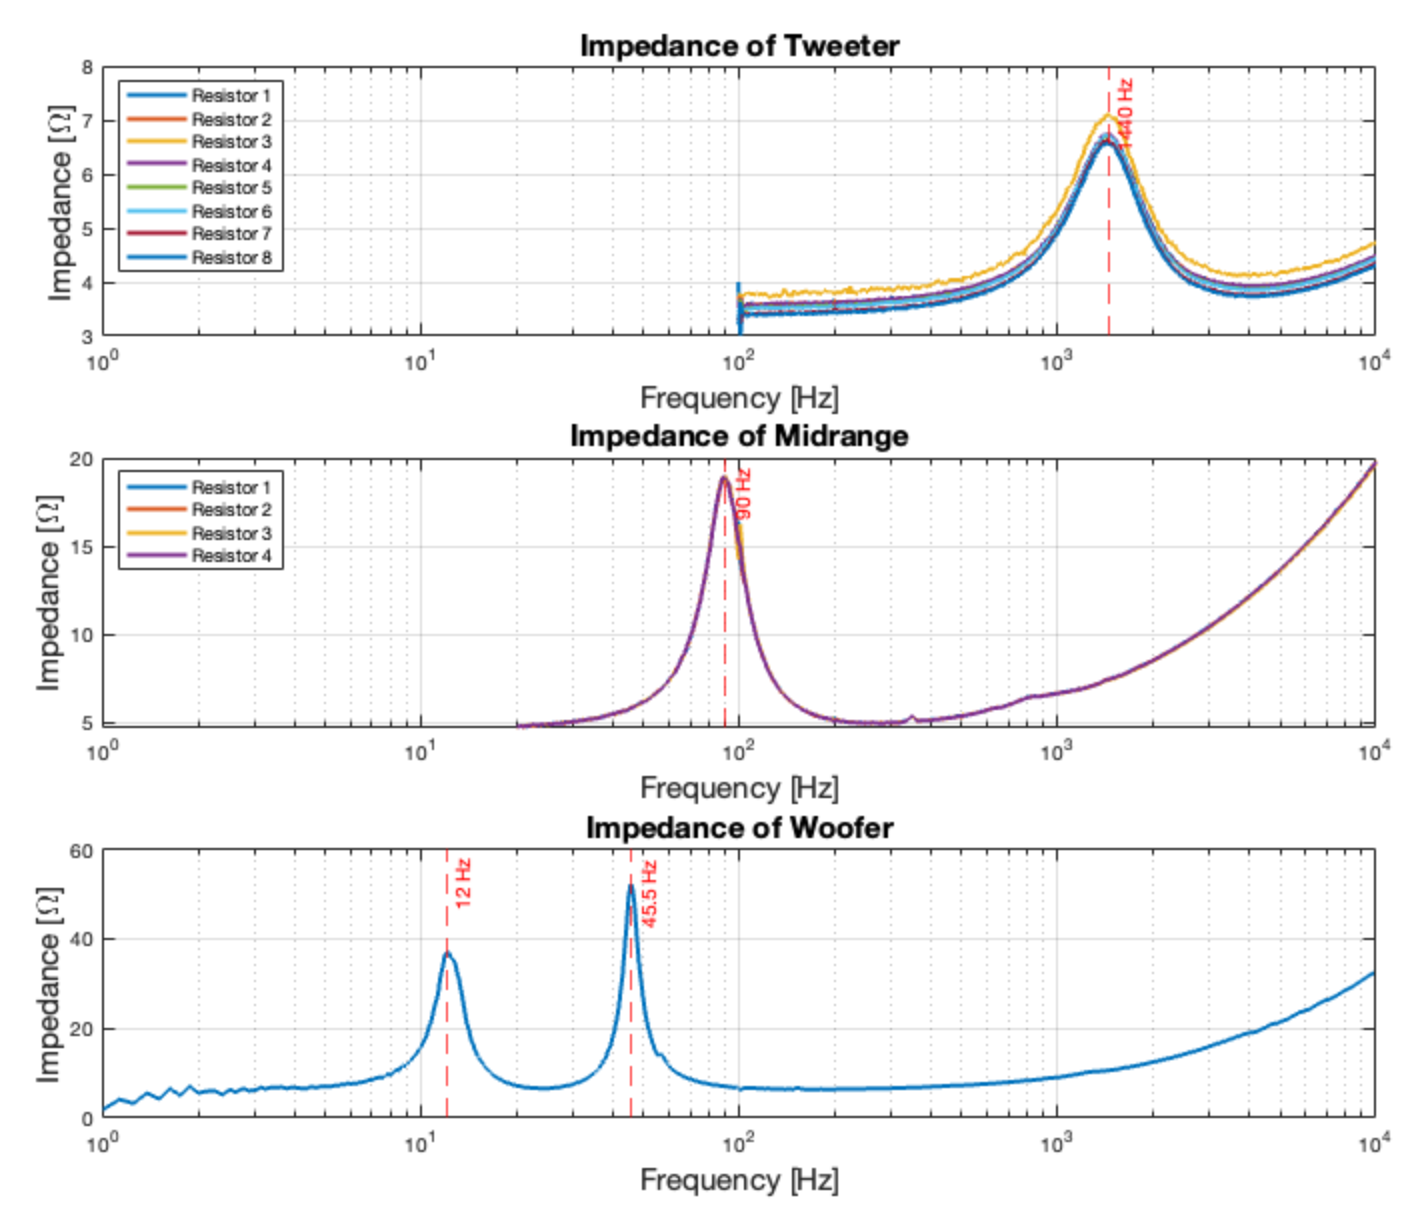
\includegraphics[width=0.6\linewidth]{Lab D/figures/Impedance_Full.png}
    \caption{Impedance for all three drivers}
    \label{fig:Impedance_Full}
\end{figure}


\subsubsection{Tweeter}

The following measurement parameters are used to assess the electrical input impedance of the tweeter:

\begin{itemize}
    \item[] f1 = 100
    \item[] f2 = 24000
    \item[] n\_oct = 48
    \item[] fres = 0.125
    \item[] Nav = 1
\end{itemize}



The tweeter impedance curves can be found in Figure \ref{fig:Impedance_Full} and show a sharp resonance around 1440 Hz at an average of 6.75 $\Omega$. The lower frequencies can be seen to trend towards  around the $R_E$ of the tweeter at 3.4 $\Omega$.


\subsubsection{Midrange}
The midrange driver had the same parameters as the tweeter, but with a frequency range going from 20 to 20000Hz. These results are also shown in Figure \ref{fig:Impedance_Full} and can be seen trending towards the midrange $R_E$ of around 4.6$\Omega$ in the low frequencies.

\subsubsection{Woofer (Open vent)}
The woofer with the open vent also uses the same parameters as the other two, but with an evaluated frequency range from 1 to 10000Hz. Figure \ref{fig:Impedance_Full} shows two sharp resonances 12Hz and 45.5Hz, and a trend towards the woofer $R_E$ of 5.7$\Omega$ in the low frequencies. These two resonances indicate that there are two systems at play when the vent is open, as both the box resonance and the vent resonance contribute to the impedance. Both of these resonances are lower than the ones for midrange and tweeter.

\subsubsection{Comparison}

Across the three drivers, there is a significant difference in impedance resonance frequency and also impedance magnitude. The woofer shows the largest impedances at the lowest frequencies, with the midrange in the middle, and the tweeter with the highest resonant frequency at the lowest magnitude.




\subsection{Thiele-Small parameters of the woofer}

\begin{figure}[H]
    \centering
    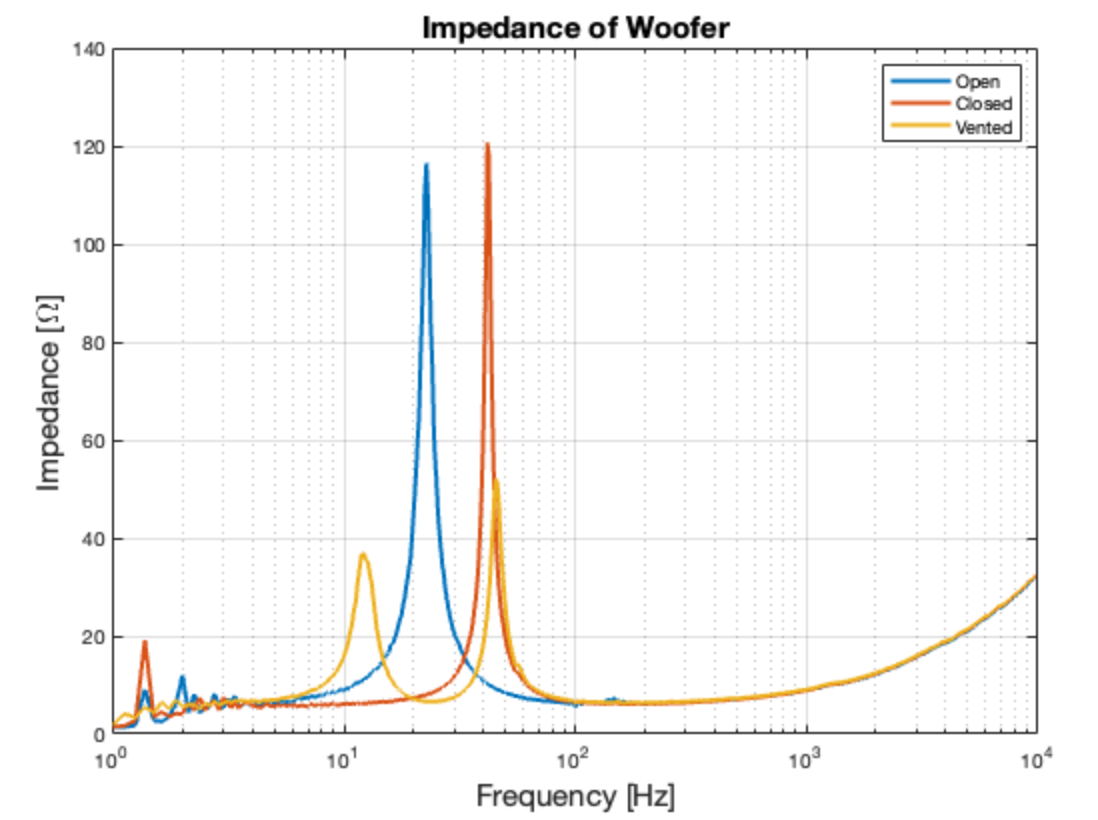
\includegraphics[width=0.5\linewidth]{Lab D/figures/Impedance_Woofer.png}
    \caption{Impedance of Woofer}
    \label{fig:Impedance_woofer}
\end{figure}

\begin{table}[H]
    \centering
    \begin{tabular}{c|c|c|c}
         & $Q_M$ & $Q_E$ & $Q_T$  \\
         \hline
        Free air & 8.8 & 0.5 & 0.48\\
        \hline
        Closed box & 18 & 0.9 & 0.86\\
        \hline
    \end{tabular}
    \caption{Q values for woofer}
    \label{tab:Qvalues}
\end{table}


\subsubsection{Free air}




\subsubsection{Closed box}

\subsubsection{Box volume}

The box volume is calculated from the equivalent volume $V_{AB}$. In this case, the filling was removed so that $V_{AB}$ is just the measured inside dimensions. The ratio between the resonant frequency for the open box $f_s$ and the resonant frequency for the closed box $f_c$ was then used from the earlier parts to calculate $V_{AS}$ as shown in the equation:

\begin{align}
    V_{AS} &= V_{AB} [(\frac{f_c}{f_s}) - 1]\\
    & = 0.215 cm^3
    \label{Vas}
\end{align}


\subsubsection{Vent influence}

\begin{table}[H]
    \centering
    \begin{tabular}{c|c|c|c}
         & 0.16m & 0.20m & 0.24m \\
         \hline
        Measured & 24.1 & 22.3 & 20.9\\
        \hline
        Calculated & 26.5 & 23.7 & 21.6\\
        \hline
        Measured: Near field & 22.75 & 21 & 19.6\\
        \hline
    \end{tabular}
    \caption{Vent resonant frequencies}
    \label{tab:ventf}
\end{table}

The vent resonant frequencies are measured by finding the minima between the two resonance peaks. They are also calculated analytically with the equation:

\begin{equation}
    f_b = \frac{c}{2 \pi} \sqrt{\frac{S}{V_{AB} L}}
    \label{eq:ventfrequency}
\end{equation}

for three different vent lengths $L$. These results are shown in Table \ref{tab:ventf}. While there is a 1-2dB difference between the measured and calculated resonance frequencies, the trend towards lower resonant frequencies with larger vent length is followed by both.

\section{Part 3: Near Field responses of the woofer unit and the vent}

Anechoic conditions are hard to fulfill below 100Hz in anechoic chambers. Therefore, near field techniques can be used at low frequencies, where the radiation impedance is dominated by the mass of air, $M_{A1}$. It follows that the sound pressure in front of the diaphragm is:

\begin{align}
    p_{near} = j \omega M_{A1} U\\
    M_{A1} = \frac{8 \rho}{3 \pi^2 a}
\end{align}

Thus, the near field pressure is a scaled up version of the frequency response at the far field pressure. To get the near field pressure, the microphone is connected to the Nexus amplifier. The output gain is set to 1 V/Pa, and the Nexus output is connected to the input channel 1 on the NI 4431. The resistor on the connection board is replaced by a short circuit. The parameters remain the same as the woofer input impedance measurements, and the transfer function between the microphone output and loudspeaker signal is calculated from the measurements.

\subsection{Vent influence}

\begin{figure}
    \centering
    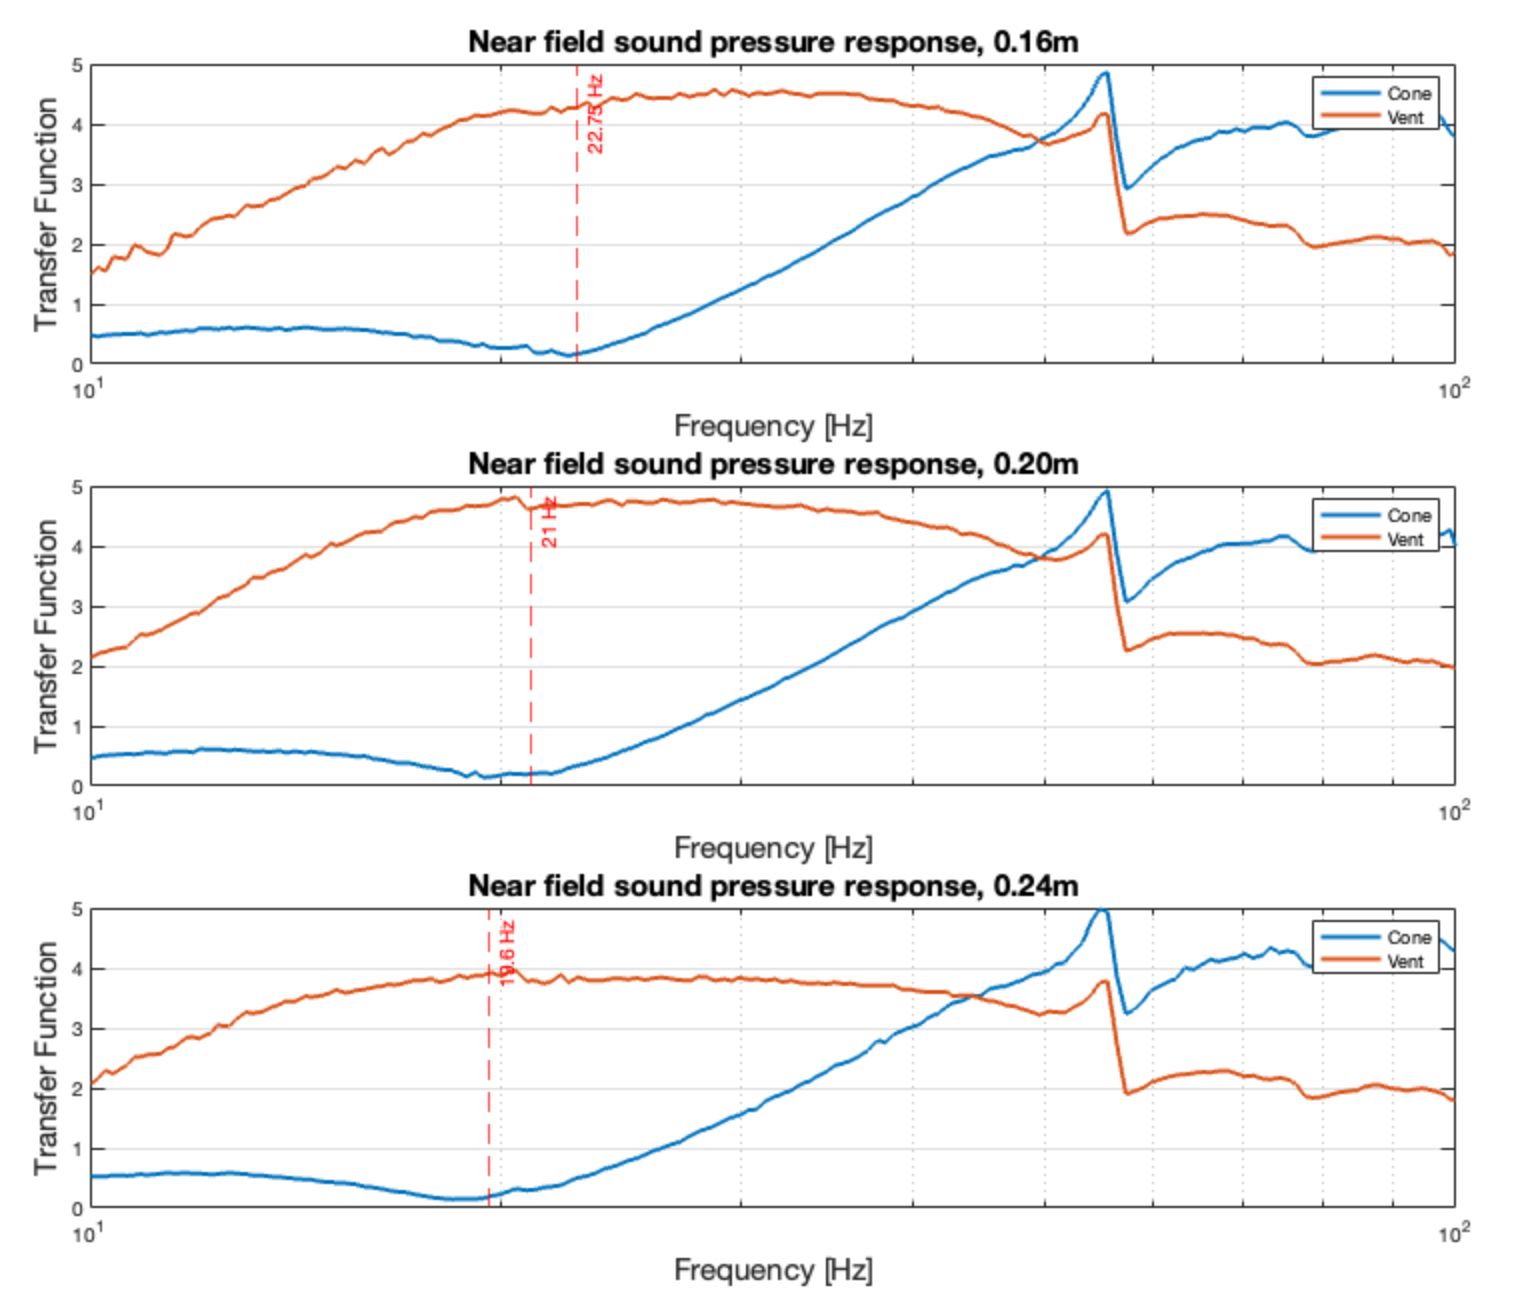
\includegraphics[width=0.8\linewidth]{Lab D/figures/NF_TF.png}
    \caption{Near field sound pressure response by vent length}
    \label{fig:NF_TF}
\end{figure}

The near field sound pressure response for each of the three tube lengths are found in Figure \ref{fig:NF_TF}. The $f_b$ is then determined by finding the peak at the vent. This peak is not the traditional sharp peak, but a very smoothed curve due to noise, a non-anechoic room, and imprecision in setting up the microphone in front of the vent and cone. The frequency at which the sound pressure in front of the vent reaches a maximum should therefore happen at the same frequency at which the sound pressure at the cone reaches a minimum. This is because the vent is at its resonance, and so it dominates the motion of the air, leaving very little air to be expelled from the cone, and most of it at the vent. It is observed that the cone response has a somewhat more pronounced dip than the vent has a peak, and this was used alongside an estimation of the vent response to estimate the vent resonance impedance frequency.\\

It can also be observed that the vent length does show a difference in 


\section{Results for loudspeaker project}

\subsection{Thiele-Small parameters of the woofer unit for the low frequency design of woofer box with vent}

\subsection{Near field measurements for woofer circuit analogy validation}

\subsection{Midrange and tweeter responses}






\end{document}